\documentclass[11pt,a4paper]{article}

\usepackage[T1]{fontenc}
\usepackage[utf8]{inputenc}
\usepackage{lmodern}
\usepackage{amsmath}
\usepackage{graphicx}
\usepackage{booktabs}
\usepackage[margin=2.5cm]{geometry}
\usepackage[hidelinks]{hyperref}

\newcommand{\brho}{$B\rho$}
\newcommand{\dedx}{$\mathrm{d}E/\mathrm{d}x$}
\newcommand{\sqdedx}{$\sqrt{\mathrm{d}E/\mathrm{d}x}$}
\newcommand{\code}[1]{\texttt{#1}}

\title{Particle identification for the a1975 deuterium-target runs:\\
estimators, calibration and the adopted recipe}
\author{Y. Ayyad}
\date{2 November 2026}

\emergencystretch=3em

\begin{document}
\maketitle

\begin{abstract}
This note documents the particle-identification (PID) study carried out on the a1975 AT-TPC runs with a
300~torr D$_2$ target and a 184~MeV $^{16}$C beam at 2.85~T, between 30 October and 2 November 2026. Three
estimators of the magnetic rigidity (\brho) and the specific energy loss (\dedx) were compared on data and on
simulations of every species that has to be separated. The dominant improvement is the gain calibration (per run
and per pad). The adopted PID uses the Spyral estimator, corrected for one failure mode -- slow elastic deuterons
emitted near 90$^\circ$ whose Spyral \brho{} is about twice too large -- by a cross-check against a
three-dimensional circle fit, and two track-quality cuts derived from the track range and the charge profile.
Deuterons and protons are separated at all \brho; tritons are separated from deuterons above 0.35~T\,m and are
confirmed independently of \dedx{} by their range. The recipe is implemented in ATTPCROOT as options of
\code{AtPIDTask} and \code{AtHelix3D}, all off by default, and was validated track by track against the analysis
macros.
\end{abstract}

\tableofcontents

\section{Introduction}

The a1975 experiment studies $^{16}$C on deuterium in inverse kinematics. The light ejectiles of interest are
deuterons (elastic scattering), protons ($^{16}$C(d,p)) and tritons ($^{16}$C(d,t)); $^4$He is also present. The
PID combines the curvature of the track in the 2.85~T field, which gives the rigidity $B\rho = p/(ze)$, with the
ionisation along the track. Because $\mathrm{d}E/\mathrm{d}x \propto z^2/\beta^2$ for the Bethe--Bloch regime,
$\sqrt{\mathrm{d}E/\mathrm{d}x}\propto z/\beta$ and
\begin{equation}
  \ln\!\left(\sqrt{\mathrm{d}E/\mathrm{d}x}\;B\rho\right) = \ln(m\gamma) + \text{const} \approx \ln m + \text{const}
  \label{eq:lnm}
\end{equation}
for $z=1$. This \emph{ln-mass} variable puts protons, deuterons and tritons $\ln 2 = 0.69$ and $\ln 1.5 = 0.405$
apart, and $^4$He ($z=2$, $B\rho = p/2$) at $\ln(m_\alpha/m_d) = 0.69$ above the deuterons. Throughout this note
the PID is shown either as the plane \sqdedx{} versus \brho{} or as the ln-mass distribution per \brho{} slice,
shifted so that the deuteron peak of each slice sits at zero.

The question that drove the study was practical: below \brho~$\approx 0.45$~T\,m the triton band was hard to see
and the different estimators disagreed on where it was.

\section{Data and simulations}

\paragraph{Data.} Reconstructed runs of the D$_2$ campaign (drift velocity 1.10424~cm/$\mu$s,
\url{/mnt/f/a1975/reco_d2_dv1104}). Calibration maps were built on runs 0017, 0019, 0021, 0022, 0027, 0031,
0032 and 0036; every comparison in this note uses four \emph{other} runs, 0016, 0026, 0058 and 0088 (107\,097
tracks with at least 30 hits), so that no calibration is judged on the data it was made from.

\paragraph{Simulations.} Three samples, digitised and reconstructed with the data parameter file:
\begin{itemize}
\item $^{16}$C(d,t)$^{15}$C, ground state and 3.103~MeV state, 20\,000 events each, gain 35\,000
  (\url{/mnt/f/a1975_C16_dt_sim});
\item d($^{16}$C,d) elastic, $4\times5000$ events, uniform in the centre-of-mass angle (2--70$^\circ$ for the
  residual), same gain (\code{C16\_dd\_el\_sim.C}, \url{/mnt/f/a1975_C16_dd_sim});
\item $^{16}$C(d,p) ground state, gain 75\,000, used for the earlier proton studies.
\end{itemize}
The elastic deuteron sample was added during this study. Without it, separation could only be judged against a
computed deuteron locus, which turned out to be misleading (Sec.~\ref{sec:dtsim}).

\section{Estimators}

Three estimators run in \code{AtPIDTask}; each fills one entry per track in \code{AtPIDEvent}.

\paragraph{Legacy (\code{AtPIDEstimator}).} Total charge over arc length. Its \dedx{} is inflated; it is kept only
for comparison.

\paragraph{Spyral (\code{AtSpyralPID}).} A port of the Spyral method: hits are sorted in $z$ (drift time), a
spline follows the track, a circle is fitted to the first arc. \dedx{} is the charge over the spline arc length on
the small pads ($\rho\le152$~mm). It gives the sharpest \dedx{} on well-measured tracks and is the default.

\paragraph{3D (\code{AtHelix3D}).} Hits are ordered in three dimensions along a minimum-spanning-tree backbone, a
helix is fitted at each end, and the vertex end is chosen by a two-out-of-three vote (rotation sense, Spyral
direction, Bragg rise). \dedx{} is the charge over the \emph{helix} path of the first arc on the small pads -- using
the zig-zag centroid polyline as path length was the main source of noise in early versions. It does not depend on
the $z$ ordering of the hits, which carries no information for tracks near 90$^\circ$.

Figure~\ref{fig:methods} compares the PID planes of Spyral and the 3D estimator before and after the gain
calibration. On the four test runs, the proton and deuteron widths in ln-mass (half width of the central 68\,\%)
went from 0.112 and 0.148 (Spyral, uncorrected) to 0.092 and 0.096 (3D, run and pad gain), and the deuteron tail
from 15.7\,\% to 8.7\,\%.

\begin{figure}[htbp]
  \centering
  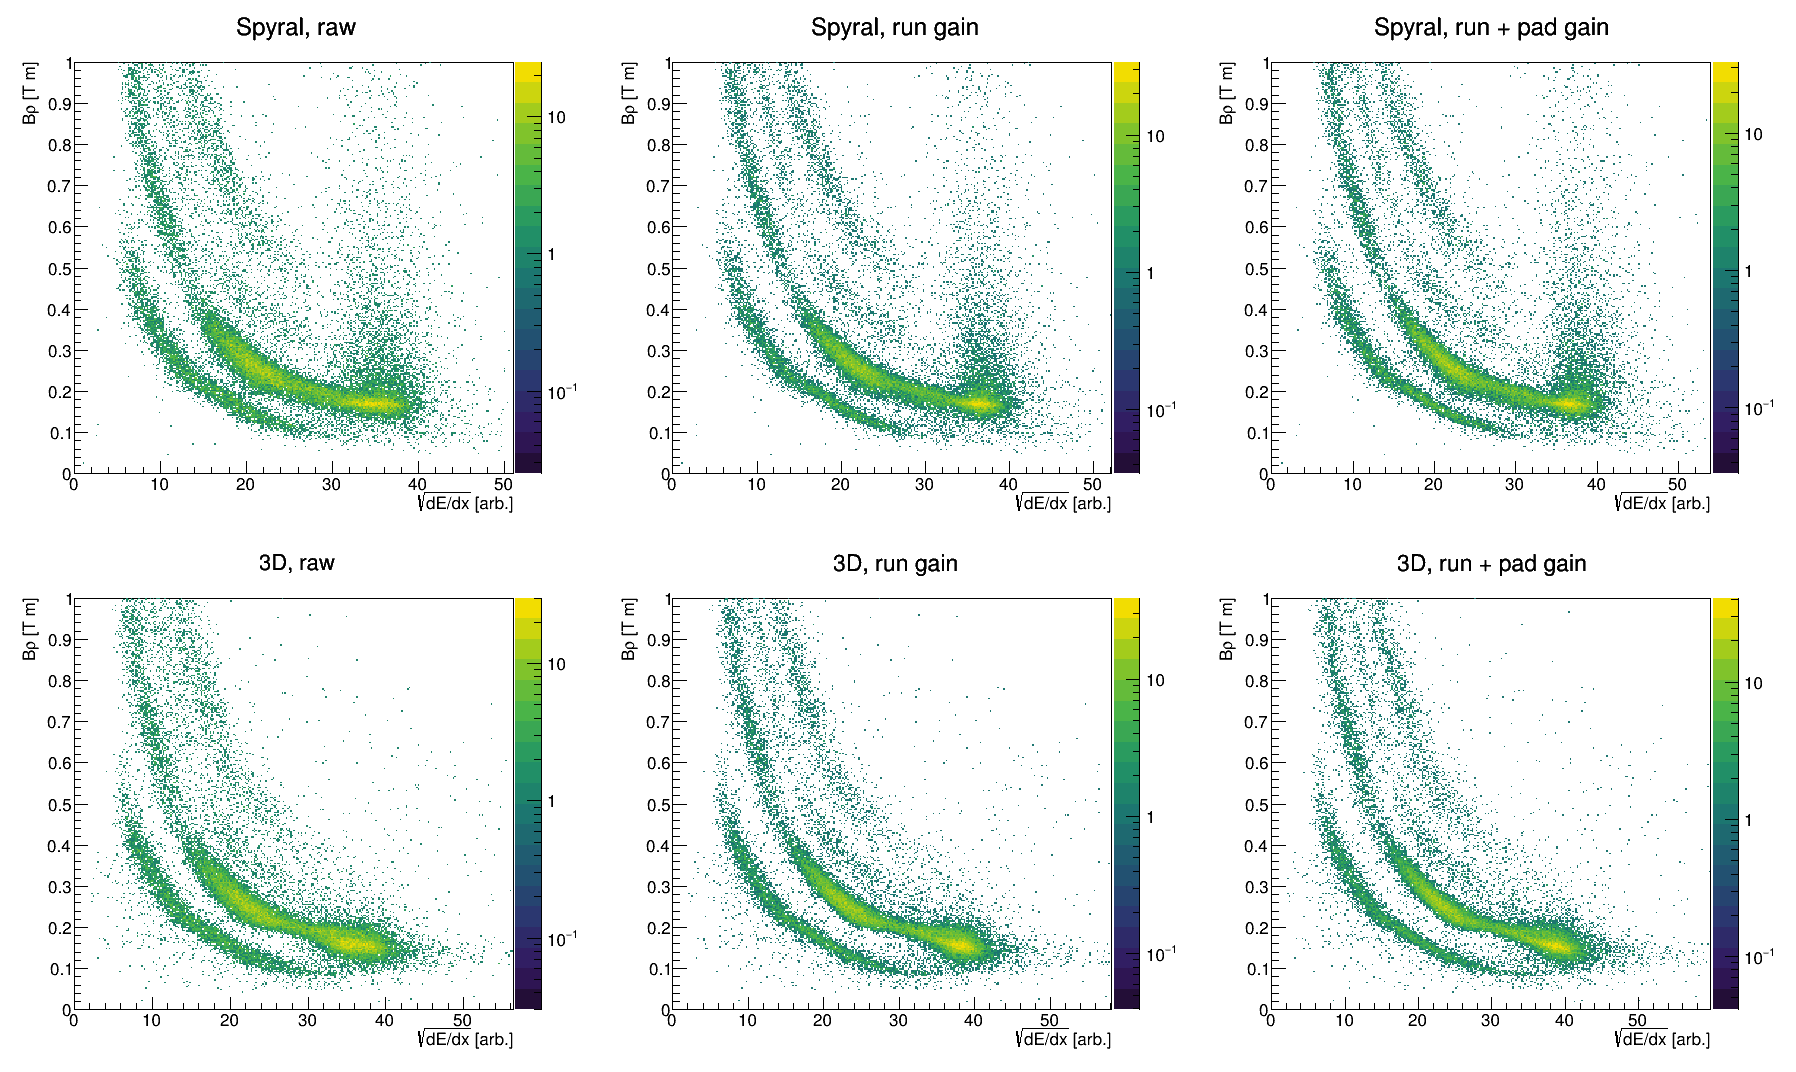
\includegraphics[width=\textwidth]{figures/pid_methods_planes.png}
  \caption{PID planes of the test runs: Spyral (top) and 3D (bottom), uncorrected, with the per-run gain, and with
  run and pad gain.}
  \label{fig:methods}
\end{figure}

\section{Gain calibration}
\label{sec:gain}

\paragraph{Per-run gain.} The deuteron band at fixed kinematics ($\theta_\mathrm{lab}$ 78--86$^\circ$,
\brho{} 0.15--0.35~T\,m, dominated by elastic deuterons) moves from 1.79 to 1.67 in ln-mass between runs 0016 and
0097: the detector gain falls by about 20\,\% over the campaign, seen identically by both estimators. Normalising
each run to a reference narrows the bands by 12--13\,\% (\code{pid\_gain\_norm.C}). In the framework the factors are
read from an \code{AtPIDGainTable} (one line per run) and applied with \code{AtPIDTask::SetDedxGain}.

\paragraph{Pad gain.} For each track, the amplitude of each small-pad hit over the track median measures the relative
gain of its pad (amplitudes above 3500~ADC excluded). The map (\code{pad\_gain\_map\_dp.C}, 6305 pads) has a 6.7\,\%
spread and a radial depression near the beam axis -- 0.78 at 20--30~mm, 0.72 at 10--20~mm, recovering by 60~mm --
that is absent in the simulation (Fig.~\ref{fig:padgain}). It is therefore a detector effect, probably
beam-induced, and is corrected. Maps from three periods of the campaign agree pad by pad (correlation 0.89--0.93);
one map is adequate. Out of sample the map narrows the bands by a further 4--7\,\%.

\begin{figure}[htbp]
  \centering
  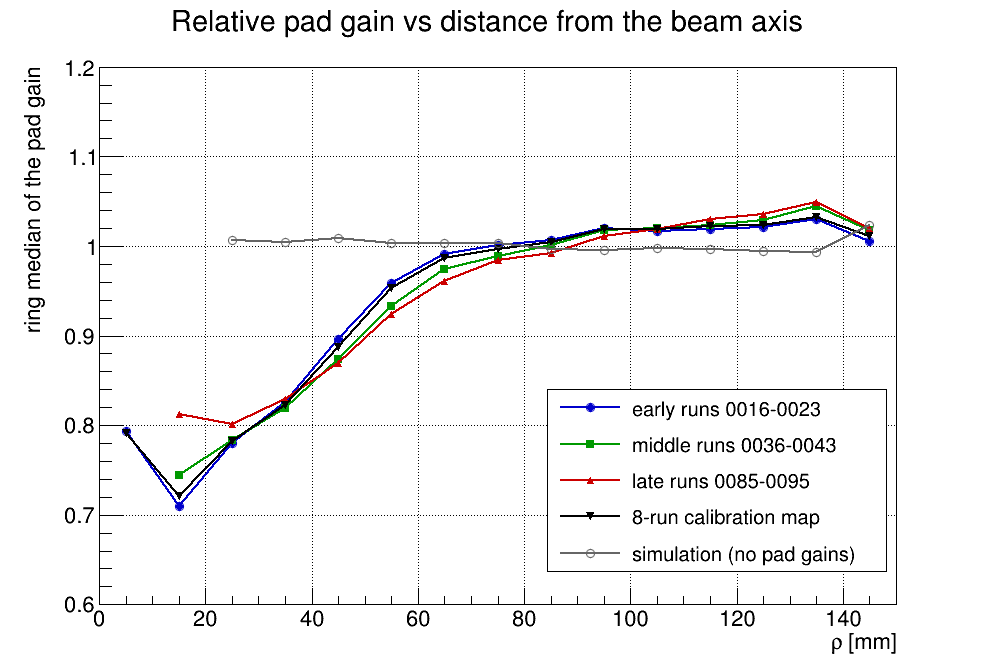
\includegraphics[width=0.7\textwidth]{figures/padgain_radial.png}
  \caption{Radial profile of the pad-gain map for three periods of the campaign. The depression near the axis is
  stable; the simulation is flat.}
  \label{fig:padgain}
\end{figure}

\paragraph{Saturation.} The GET electronics saturate. With the multi-fit PSA the hit amplitudes pile up between about
3800 and 4850~ADC (per-pad maximum 4430--4630, median 4548). On slow deuterons (\brho{} 0.15--0.20~T\,m) 77\,\% of
the tracks have saturated samples in their PID segment, about 21\,\% of the segment on average. The simulation had
no ceiling at all (simulated amplitudes reach 20\,340~ADC). An option to clip the simulated traces
(\code{AtPulse::SetADCCeiling}) was added, but its value is not fixed: the PSA extrapolates a clipped pulse to about
1.34 times the clip and the simulation then produces a spike that the data do not have (Fig.~\ref{fig:ceiling}).
The per-pad saturation shape has to be measured from the data first (Sec.~\ref{sec:open}).

\begin{figure}[htbp]
  \centering
  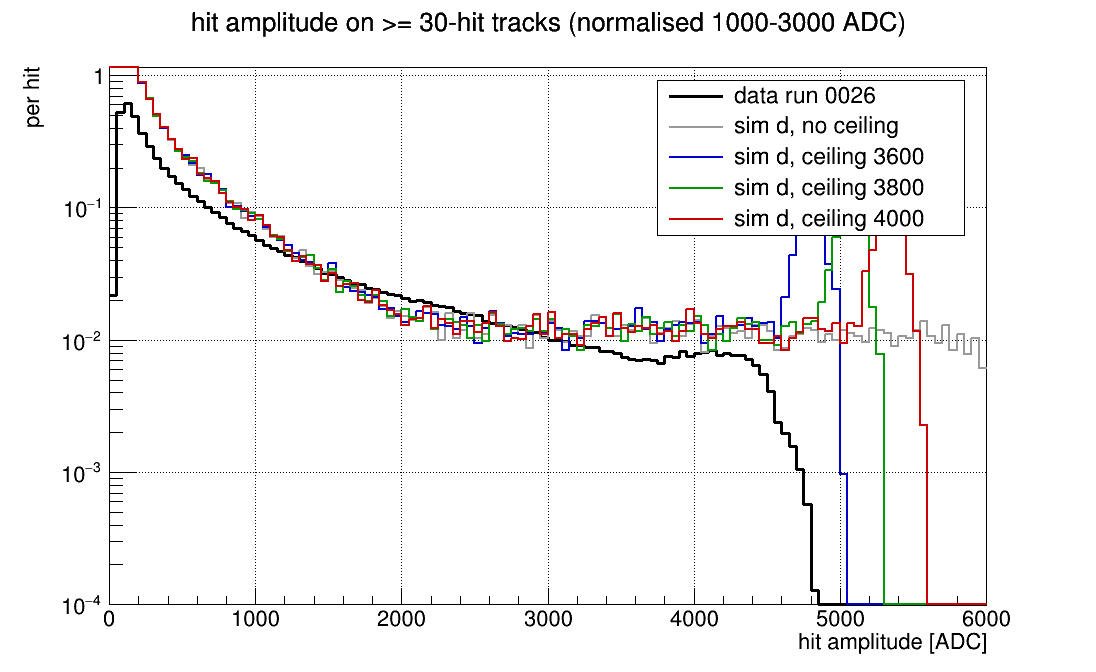
\includegraphics[width=0.75\textwidth]{figures/adc_ceiling_scan.png}
  \caption{Hit-amplitude spectrum of the data compared with the elastic-deuteron simulation reconstructed with
  trace ceilings of 3600, 3800 and 4000~ADC.}
  \label{fig:ceiling}
\end{figure}

\section{Rigidity of slow tracks}

A slowly moving particle loses a large fraction of its energy along the part of the track that is fitted, so its
helix tightens. Any single circle fitted over that stretch returns an average radius, smaller than the radius at the
vertex. The relative effect scales as
\begin{equation}
  \frac{\mathrm{d}E/\mathrm{d}x}{E} \propto \frac{m^2/p^2}{p^2/m} = \frac{m^3}{p^4},
\end{equation}
so it is 3.4 times larger for tritons than for deuterons at the same momentum, and switches on steeply below
\brho~$\approx0.45$~T\,m. On simulated tritons the 3D circle underestimates \brho{} by 13--39\,\% at true
\brho{} 0.25--0.45~T\,m, Spyral by 8--27\,\% (Table~\ref{tab:brhobias}). Spyral's smaller bias is accidental: its
radius is equally low, but its polar angle is too steep, which inflates \brho{} by 10--13\,\% and partly cancels the
radius deficit.

\begin{table}[htbp]
  \centering
  \caption{Median $\ln(B\rho/B\rho_\mathrm{true})$ for simulated tritons, with the half width of the central 68\,\%
  in brackets.}
  \label{tab:brhobias}
  \small
  \begin{tabular}{lcccc}
    \toprule
    True \brho{} [T\,m] & Spyral & 3D circle & Shrinking & Genfit \\
    & & + arc angle & radius & (triton hyp.) \\
    \midrule
    0.25--0.30 & $-0.27$ [0.07] & $-0.39$ [0.08] & $-0.33$ [0.12] & $-0.002$ [0.05] \\
    0.30--0.35 & $-0.14$ [0.06] & $-0.31$ [0.07] & $-0.09$ [0.12] & $+0.002$ [0.03] \\
    0.35--0.45 & $-0.08$ [0.03] & $-0.13$ [0.05] & $-0.02$ [0.03] & $-0.004$ [0.02] \\
    0.45--0.60 & $-0.03$ [0.02] & $-0.04$ [0.03] & $-0.01$ [0.02] & $-0.004$ [0.03] \\
    \bottomrule
  \end{tabular}
\end{table}

Several remedies were tried:
\begin{itemize}
\item \emph{Hit refit} (\code{AtHelix3D::SetHitRefit}): refit the vertex-end circle on the raw hits rather than the
  4~mm centroids. Better precision.
\item \emph{Arc-length angle} (\code{AtHelix3D::SetArcAngle}): the polar angle from $z$ against the arc length round
  the vertex-end circle, over the first half of the window. Unbiased on simulation to 0.2--0.3\,\% in
  $\sin\theta$. The arc length must use the \emph{net} phase; summing the absolute phase steps inflates it with the
  hit-order jitter. Together with the hit refit this is the recommended 3D \brho{} (\code{brhoArc}).
\item \emph{Shrinking-radius fit}: $r(\phi) = R_0 + k\phi$ round a free centre, $R_0$ being the radius at the
  vertex. It removes most of the bias down to 0.35~T\,m, but its precision degrades below that.
\item \emph{Equation-of-motion fits}, with a mass hypothesis or species-blind with the energy loss driven by the
  measured \dedx{} or by a Bragg-curve fit. Accurate on simulation, but their per-track scatter (9--25\,\% on the
  mass) gave no PID gain on data.
\item \emph{Genfit} with either hypothesis: with the correct species the vertex \brho{} is excellent
  (Table~\ref{tab:brhobias}); with the wrong one it is off by 12--21\,\%.
\end{itemize}

\section{Deuteron--triton separation tested on both species}
\label{sec:dtsim}

Early comparisons placed the simulated tritons relative to a \emph{computed} deuteron locus and concluded that the
circle pulled slow tritons onto the deuteron band. The elastic-deuteron simulation showed that this was wrong: the
circle biases slow deuterons too, so both bands move together and stay apart (Fig.~\ref{fig:dtsim}). The bend of the
deuteron band towards high \dedx{} at 0.2--0.3~T\,m is real -- deuterons stopping inside the measured segment -- and
appears in the true-\brho{} plane.

\begin{figure}[htbp]
  \centering
  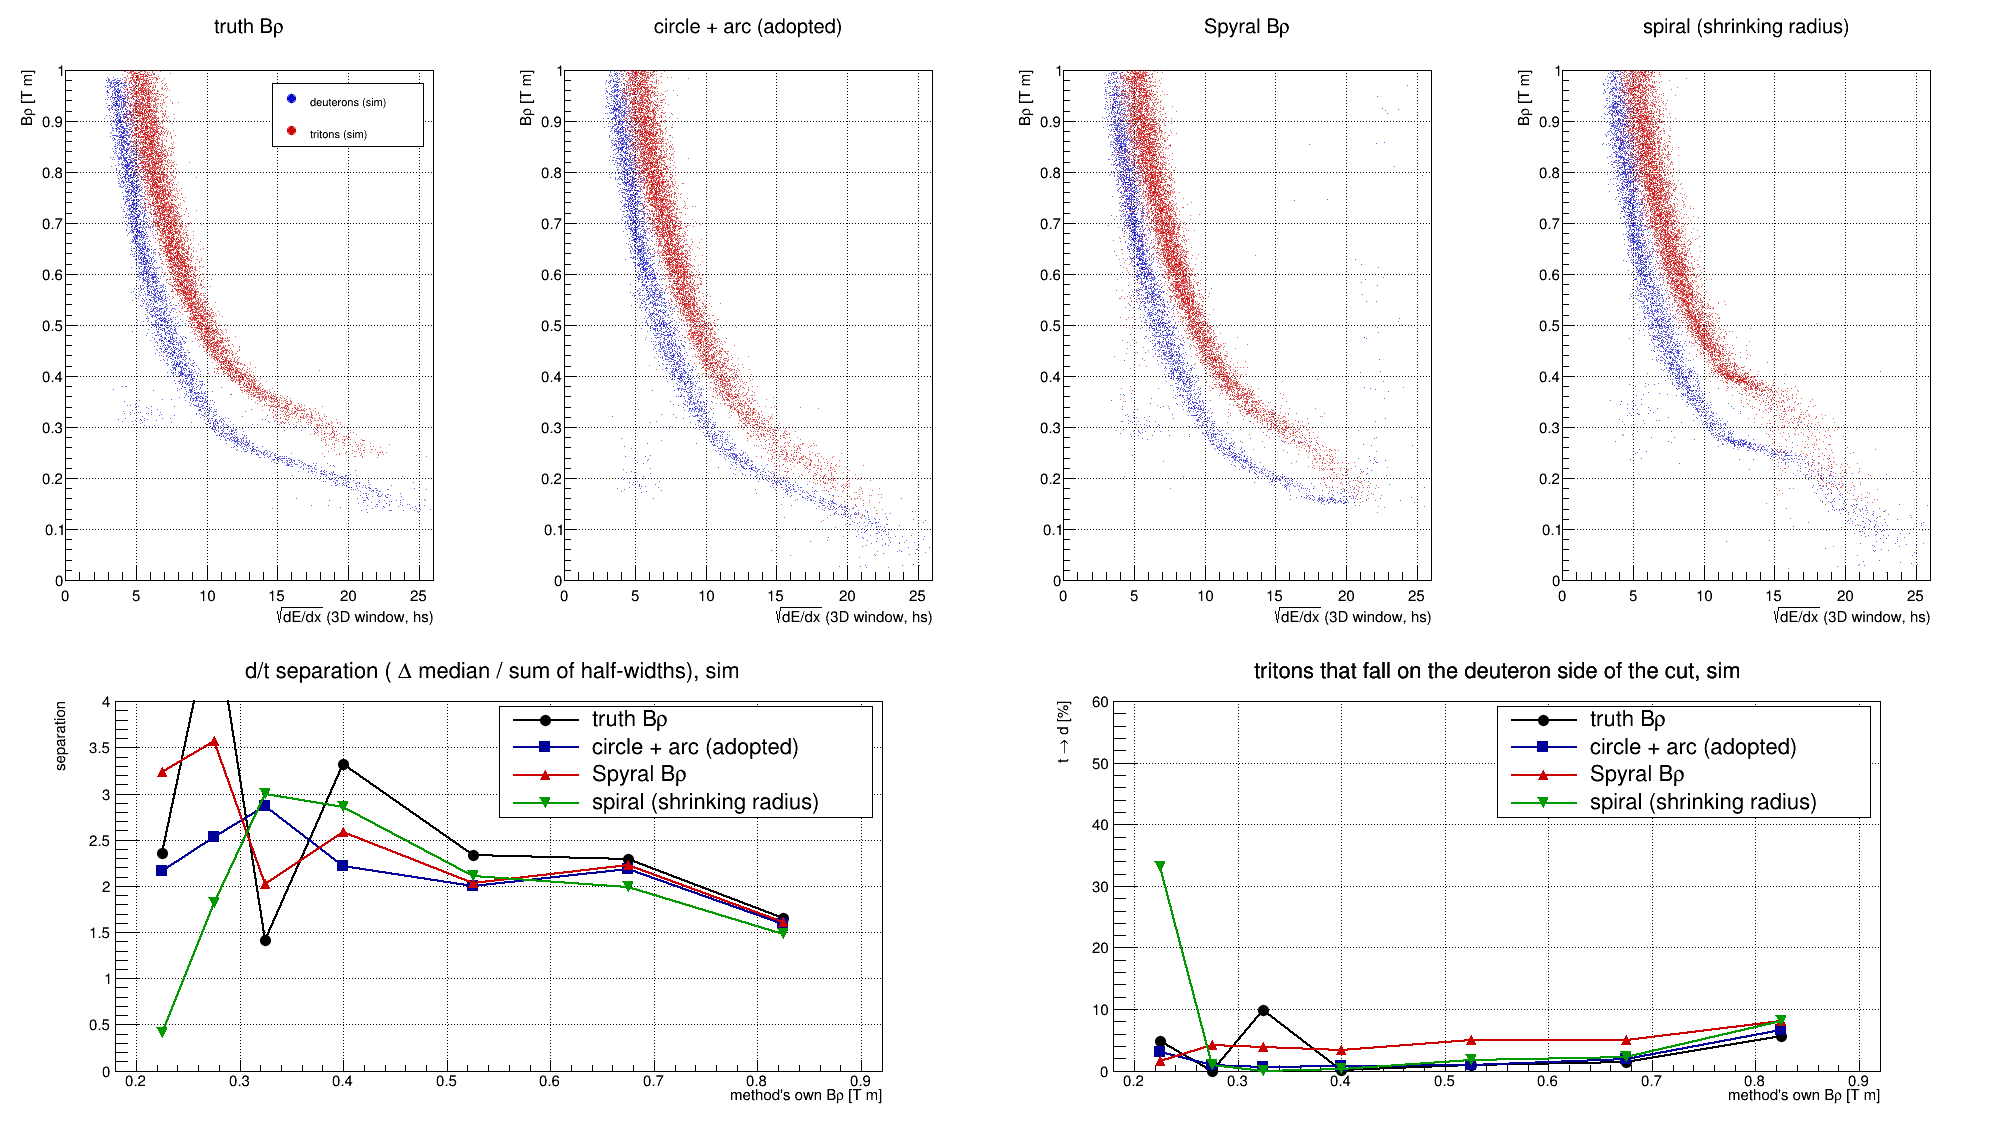
\includegraphics[width=\textwidth]{figures/pid_dt_sim.png}
  \caption{Simulated deuterons (blue) and tritons (red) in the same plane for each \brho{} estimator, with the
  separation and the fraction of misidentified tracks per slice of the estimator's own \brho.}
  \label{fig:dtsim}
\end{figure}

\begin{table}[htbp]
  \centering
  \caption{Simulated deuteron/triton separation (median difference over the sum of half widths) and
  misidentification (tritons lost / deuterons in the triton gate) per slice of each estimator's own \brho.}
  \label{tab:dtsim}
  \begin{tabular}{lccc}
    \toprule
    \brho{} [T\,m] & 3D circle & Spyral & Shrinking radius \\
    \midrule
    0.20--0.25 & 2.2; 3.0\,\% / 0.5\,\% & 3.2; 1.6\,\% / 9.7\,\% & 0.4; fails \\
    0.25--0.30 & 2.5; 0.9\,\% / 2.4\,\% & 3.6; 4.1\,\% / 9.7\,\% & 1.8; 1.0\,\% / 6.9\,\% \\
    0.30--0.35 & 2.9; 0.7\,\% / 2.1\,\% & 2.0; 3.8\,\% / 3.2\,\% & 3.0; 0.0\,\% / 6.4\,\% \\
    0.35--0.45 & 2.2; 0.8\,\% / 0.9\,\% & 2.6; 3.3\,\% / 2.3\,\% & 2.9; 0.3\,\% / 1.6\,\% \\
    \bottomrule
  \end{tabular}
\end{table}

The 9.7\,\% of simulated deuterons that Spyral puts in the triton gate at 0.20--0.30~T\,m reproduce, from truth, the
fake triton population seen on data (Sec.~\ref{sec:spyral}).

\paragraph{What limits the separation.} With genfit's \brho{} under each hypothesis, the measured \dedx{} can be
compared with the CATIMA prediction for deuterons and for tritons. The energy-loss model is consistent (correct
hypothesis within 0--5\,\%), but the two residuals move together and carry the same information as the ln-mass
variable; the misidentification is no better than with the circle, and worse above 0.45~T\,m where genfit's \brho{}
has longer tails (Fig.~\ref{fig:gf}). The genfit fit quality does not choose the species either: the triton
hypothesis fits better for 97--99\,\% of tritons but also for 63--93\,\% of deuterons below 0.35~T\,m, also with a
realistic hit uncertainty (0.6~mm). The separation is limited by the \dedx{} resolution, about $\pm5$\,\% in ln,
not by \brho. A truncated mean of the \dedx{} was worse below 0.35~T\,m -- for stopping tracks the highest samples
are the real Bragg rise -- and only marginally better above 0.45~T\,m; averaging the Spyral and 3D \dedx{} narrows the
deuteron band by at most 7\,\% because both measure the same charge. Genfit's role is the kinematics once the
species is known.

\begin{figure}[htbp]
  \centering
  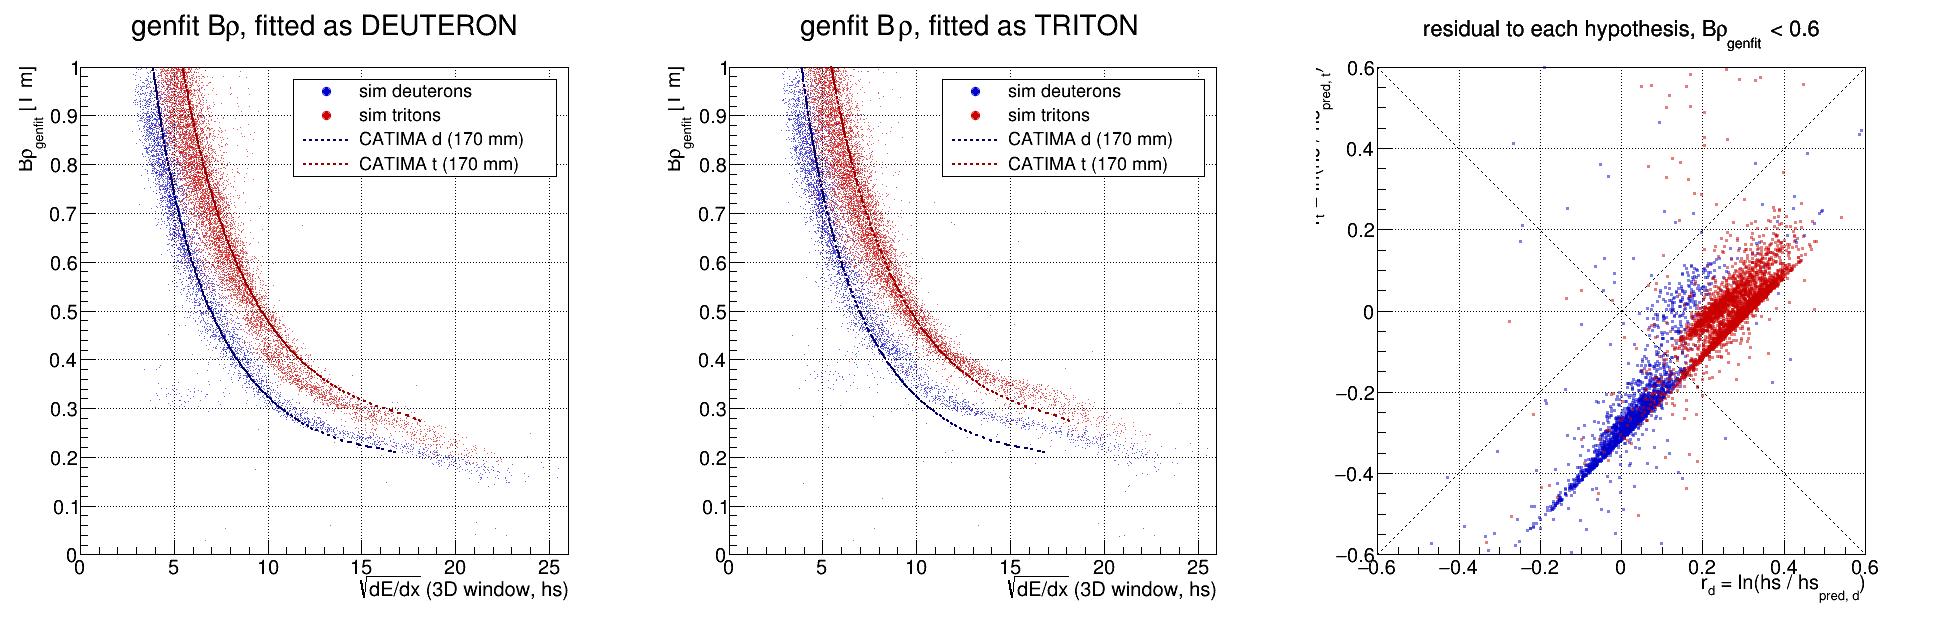
\includegraphics[width=\textwidth]{figures/pid_gf_sim.png}
  \caption{Simulated deuterons and tritons with genfit \brho{} under the deuteron and triton hypotheses, and the
  residuals of the measured \dedx{} to the prediction for each hypothesis.}
  \label{fig:gf}
\end{figure}

\section{Spyral's failure on flat tracks}
\label{sec:spyral}

On data, Spyral shows a blob at the low-\brho{} end of the deuteron band and a streak above it, which populate the
triton region (Fig.~\ref{fig:veto}, left). The tracks involved are slow elastic deuterons near 90$^\circ$: circle
\brho{} 0.14~T\,m, about 100 hits, a $z$ extent of only $\sim10$~mm, 99\,\% stopping in the gas. In the circle PID
66\,\% of them are in the deuteron band and they show no triton excess; their energy agrees with the elastic
kinematics for the circle (with the usual deceleration bias) and not for Spyral (1.9 times too high, with a large
spread). The cause is Spyral's radius, 1.6 times the circle's, while the two agree within 1\,\% for other tracks at
the same \brho: a track spanning a few time buckets gives Spyral's $z$-ordered spline almost no ordering
information.

The veto drops Spyral's result when
\begin{equation}
  \ln\frac{B\rho_\mathrm{Spyral}}{B\rho_\mathrm{circle}} \ge 0.25
  \quad\text{and}\quad
  \left(B\rho_\mathrm{Spyral} < 0.45~\mathrm{T\,m}\ \text{or}\ \sqrt{\mathrm{d}E/\mathrm{d}x} > 30\right),
\end{equation}
the second condition catching the upper part of the streak, which extends to 0.9~T\,m at high \dedx. It removes 14\,\%
of the tracks and keeps 97.5--100\,\% of simulated tritons above circle \brho{} 0.25~T\,m. The vetoed tracks are then
re-added with the circle \brho{} and the 3D \dedx{} scaled to the Spyral scale (factor 0.965, the median ratio where
the two \brho{} agree); 95\,\% of them land on the end of the deuteron band (Fig.~\ref{fig:final}).

\begin{figure}[htbp]
  \centering
  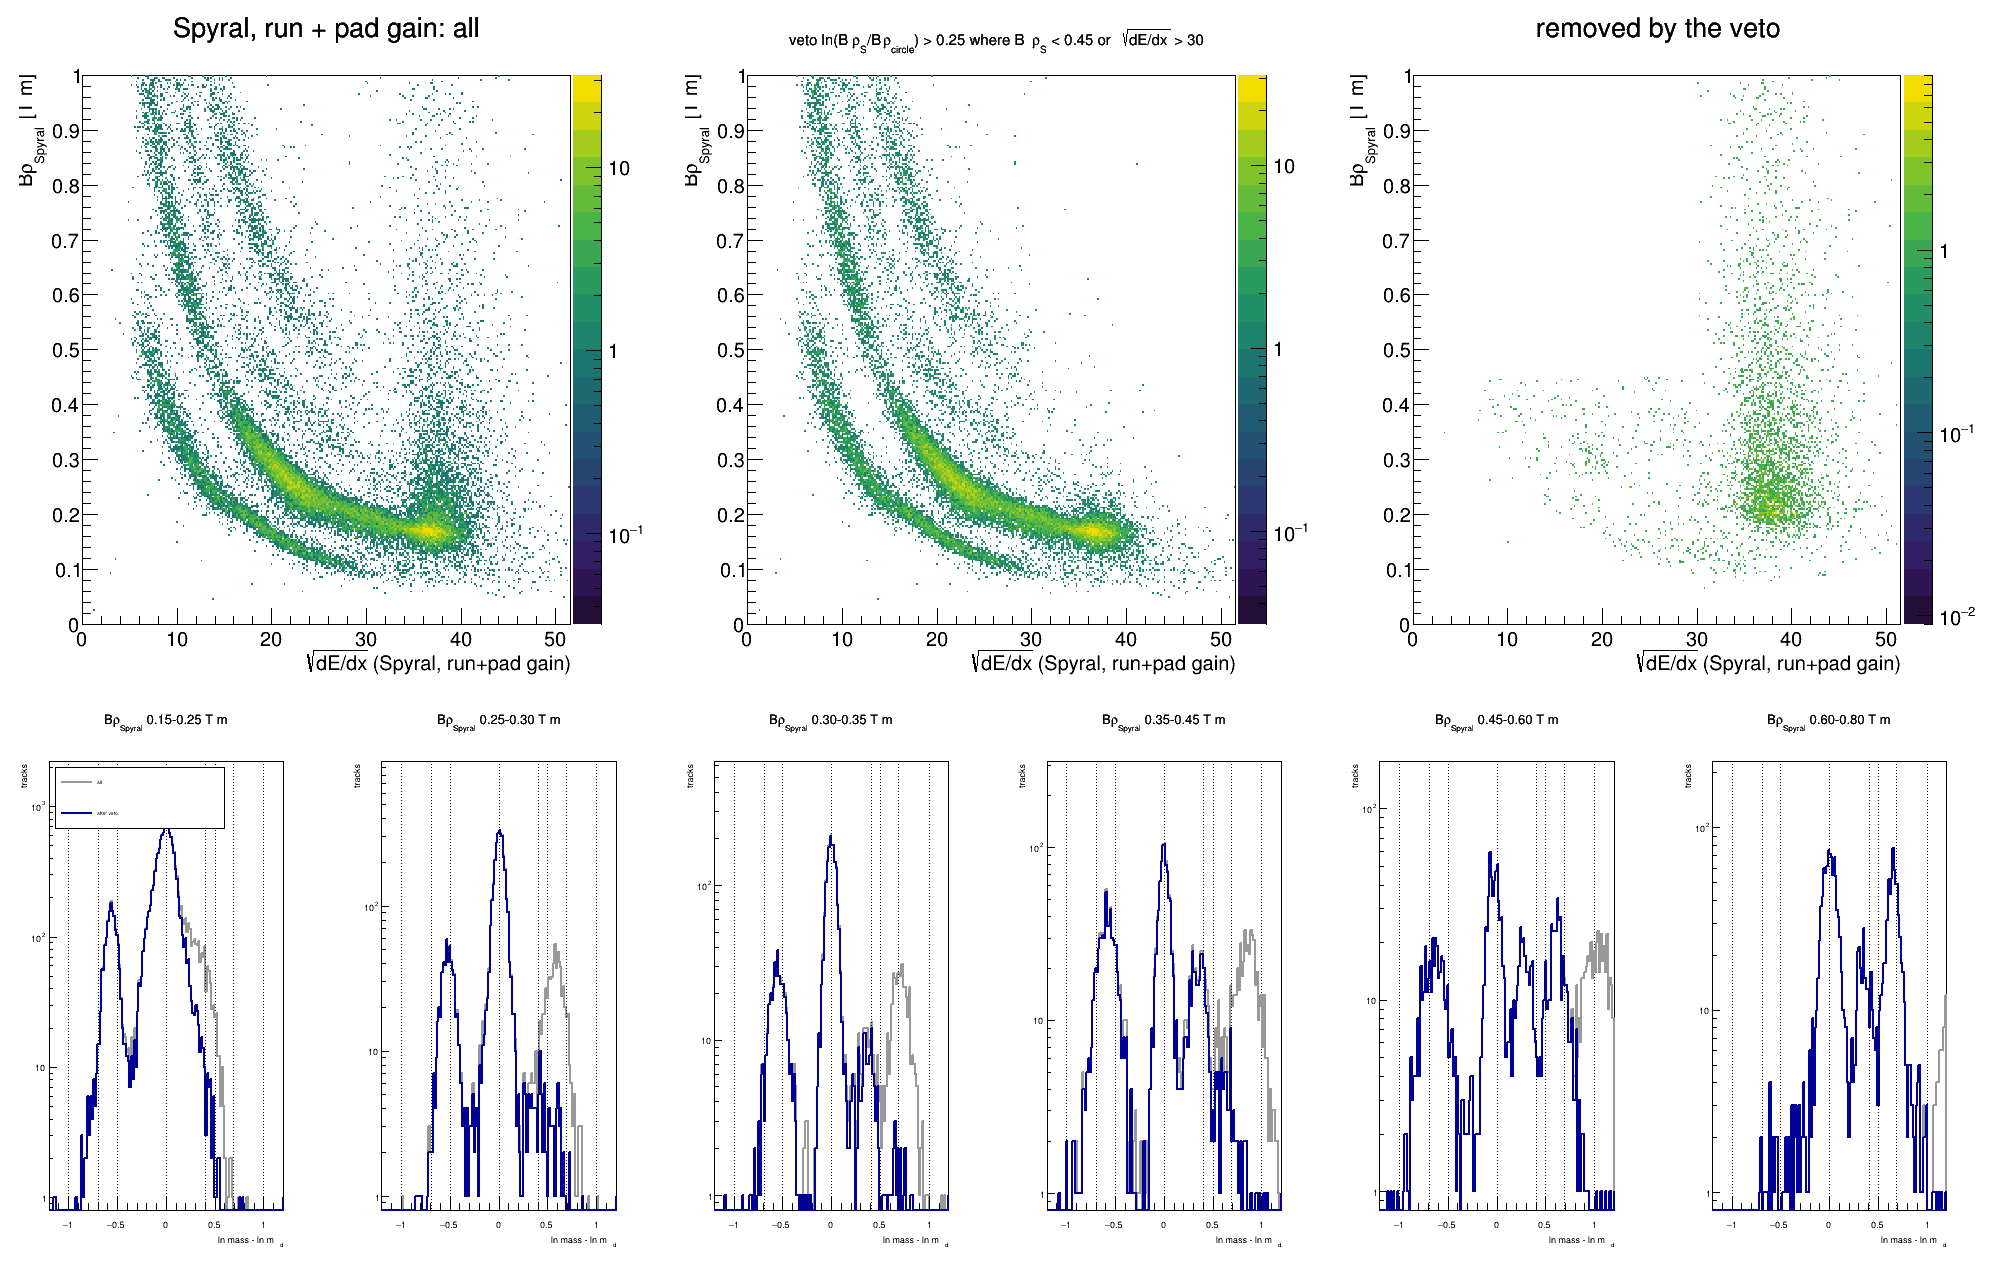
\includegraphics[width=\textwidth]{figures/pid_spyral_veto_opt2.png}
  \caption{Spyral PID before the veto, after it, and the vetoed tracks; bottom: ln-mass per Spyral-\brho{} slice
  before (grey) and after (blue).}
  \label{fig:veto}
\end{figure}

\section{Range and track quality}

For a track that stops in the gas, the range at fixed \brho{} scales as $z^2 (B\rho)^4/M^3$: a triton's range is
about 0.3 of a deuteron's at the same momentum, and no $z=1$ or $z=2$ ion stops shorter than a triton. Range does not
depend on the gain or on saturation. A track is taken as stopping when its far end lies within 145~mm of the axis and
between 10 and 955~mm in $z$; the upper limit matters, because tracks leaving the end of the drift window
($z\approx964$~mm) otherwise look contained.

On simulation, range alone separates less well than \dedx{} (the circle bias differs between the species, so the
gap at fixed circle \brho{} is about 0.5 rather than 0.3), and combined with \dedx{} it helps only at
0.25--0.45~T\,m. On data, however, the range plane (Fig.~\ref{fig:range}) shows the proton, deuteron and triton
bands on the simulated curves, which confirms the tritons at 0.25--0.45~T\,m independently of \dedx.

\begin{figure}[htbp]
  \centering
  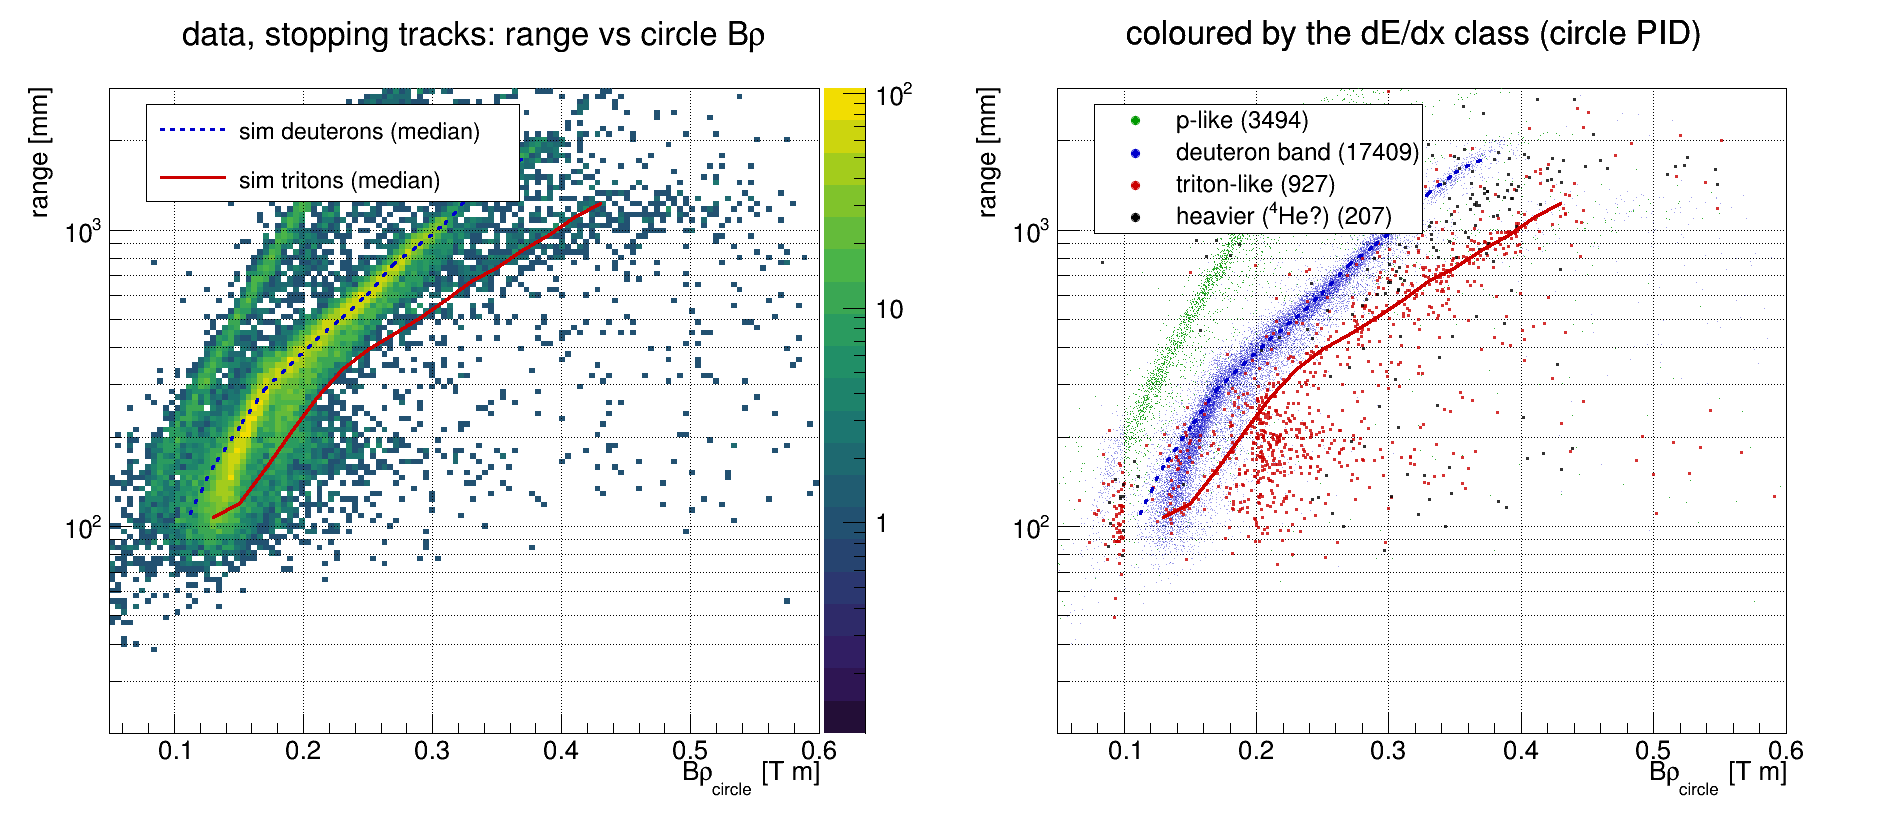
\includegraphics[width=\textwidth]{figures/pid_range_data.png}
  \caption{Range against circle \brho{} for stopping tracks in the data, with the simulated deuteron and triton
  medians; right: coloured by the \dedx{} class of the circle PID.}
  \label{fig:range}
\end{figure}

Of the data tracks in the triton region of \dedx{} at \brho{} 0.15--0.45~T\,m, only 3--9\,\% have a deuteron range,
30--54\,\% lie on the triton curve, and 26--58\,\% are \emph{shorter} than any triton. An automatic classification of
the 301 short ones (\code{classify\_short\_t\_dp.C}, Fig.~\ref{fig:short}) finds that 67\,\% have their charge peak well
before the end of the candidate with only weak charge after it: a stopped particle to which the track finder attached
other hits. The rest are a mix of real tritons in the short tail of the range distribution, short nearly straight
tracks with saturated charge, and blobs.

\begin{figure}[htbp]
  \centering
  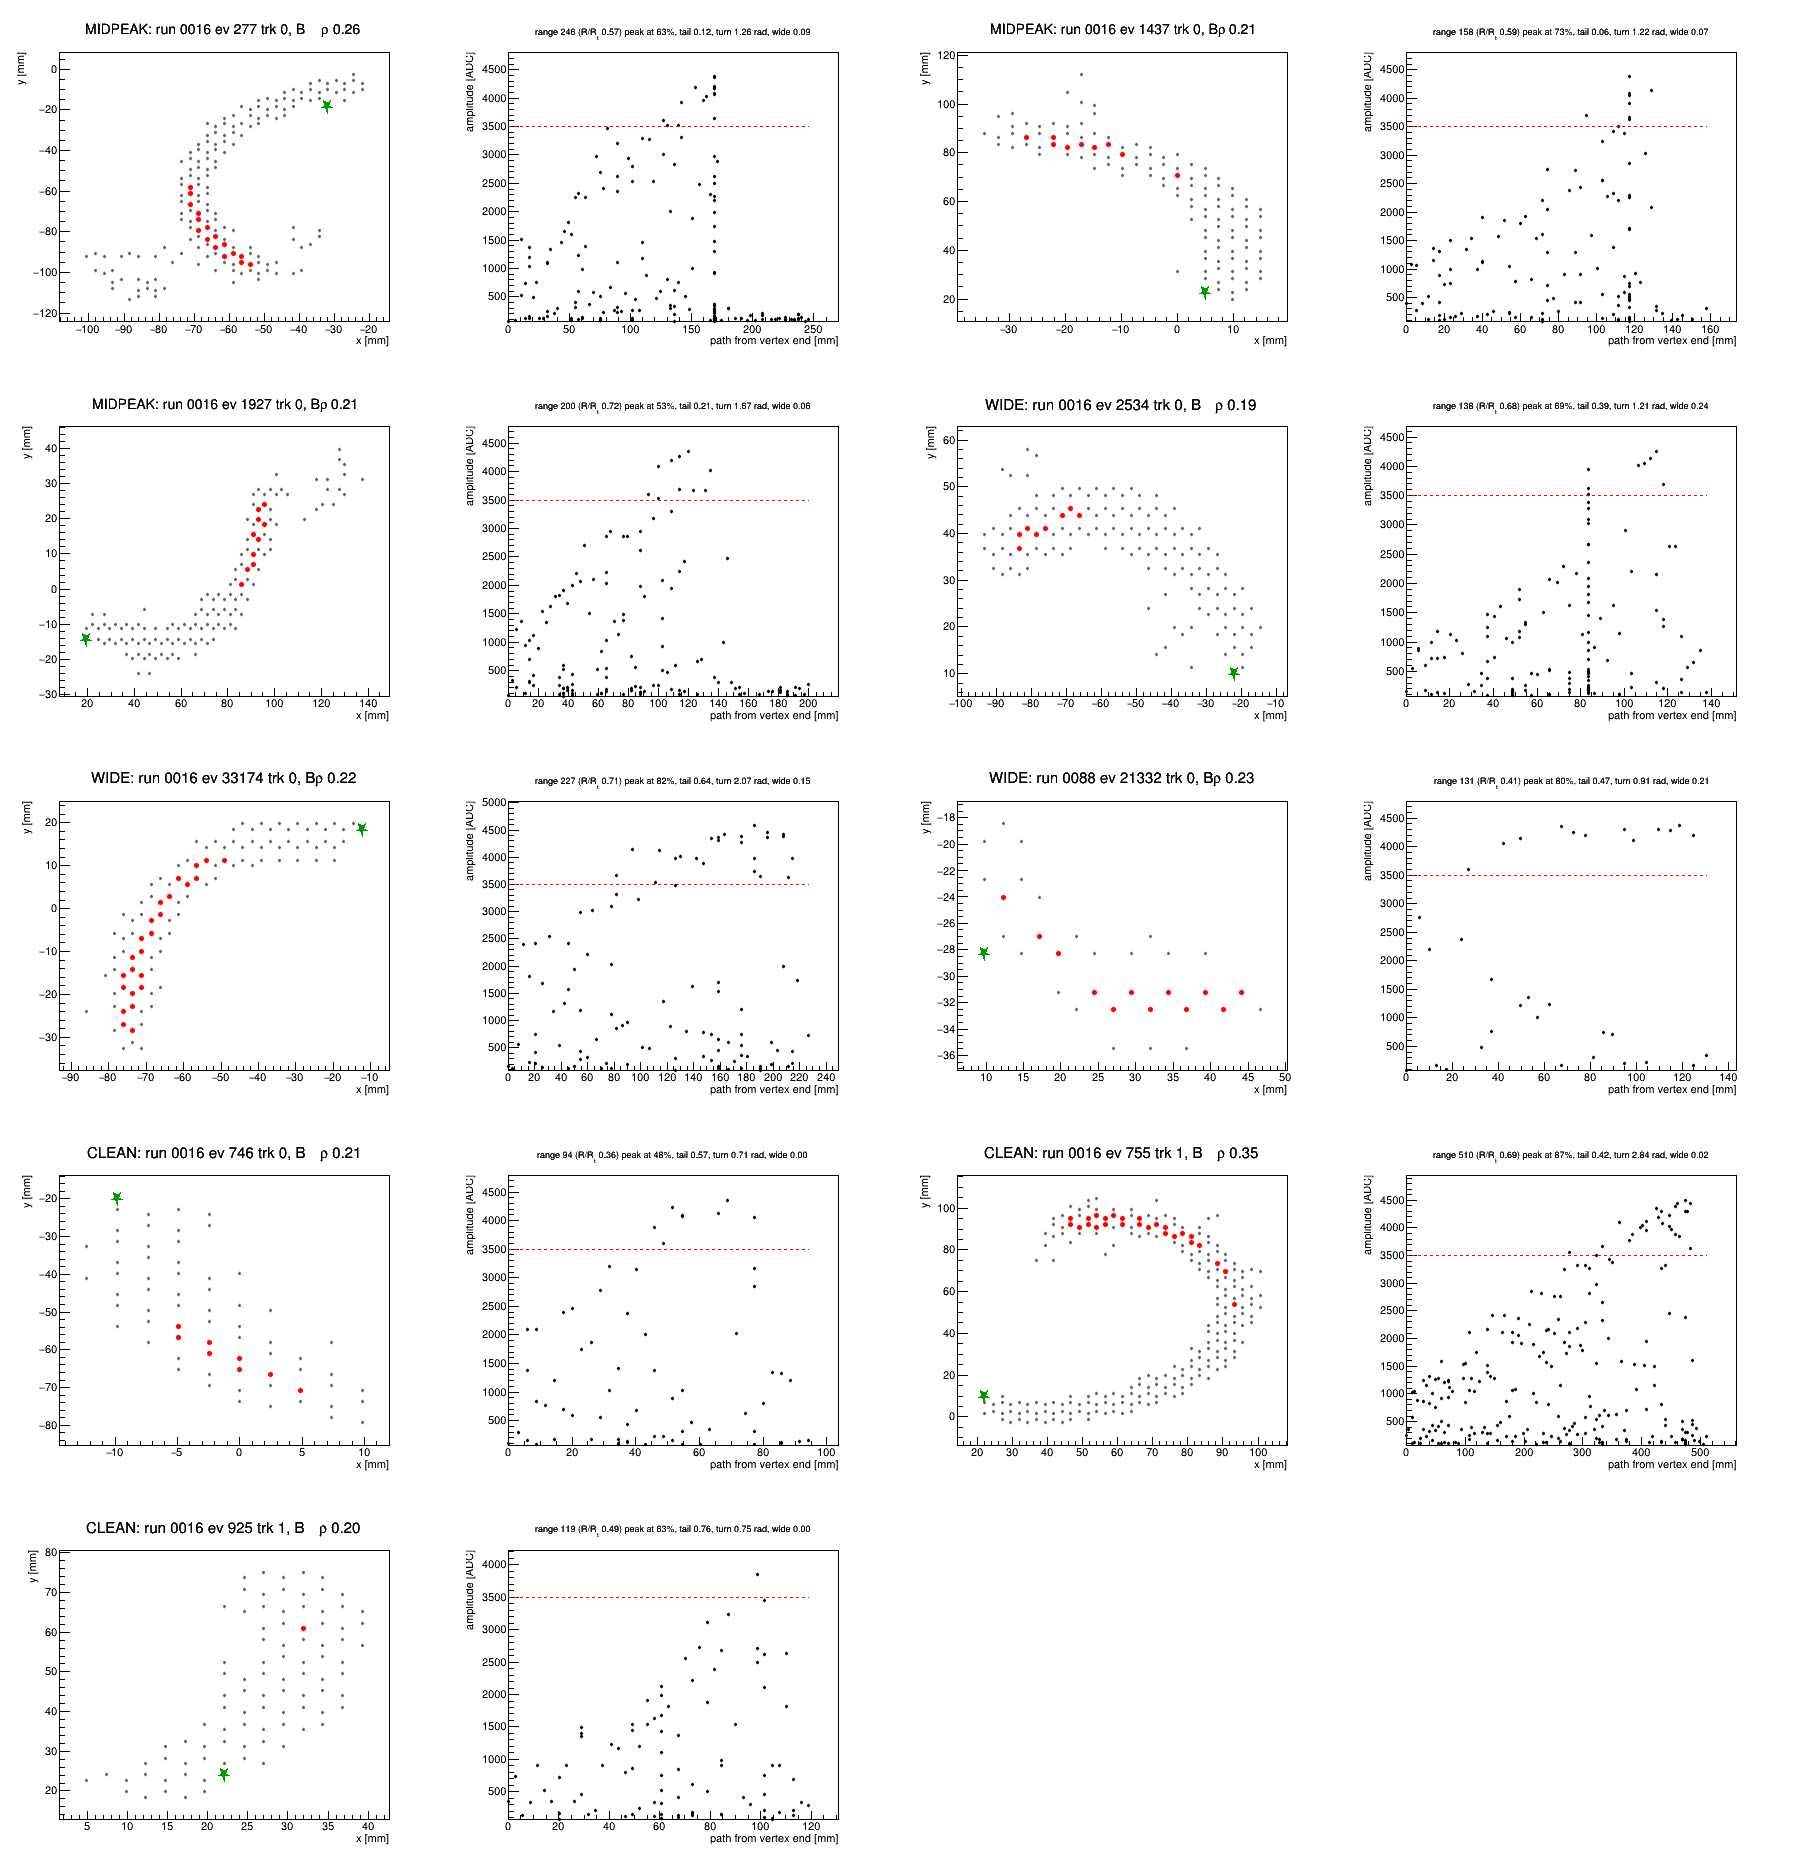
\includegraphics[width=\textwidth]{figures/short_t_examples.png}
  \caption{Examples of short triton-like tracks by class: $xy$ view (saturated hits red, vertex end marked) and
  amplitude along the track.}
  \label{fig:short}
\end{figure}

Two quality cuts follow, applied to stopping tracks:
\begin{itemize}
\item \emph{too short}: range below $e^{-0.4}$ times the simulated triton range at the circle \brho{}
  (0.13--0.44~T\,m), species-blind;
\item \emph{mid-track charge peak}: the charge profile (10~mm bins) peaks before 75\,\% of the track, more than
  30~mm before its end, and the mean after the peak is below 35\,\% of it -- applied only in the triton region
  (0.20--0.60 above the deuteron peak in ln-mass). Applied everywhere it would also remove 17\,\% of the slow
  deuterons at 0.10--0.15~T\,m.
\end{itemize}

\section{Adopted PID and performance}

The adopted PID is:
\begin{enumerate}
\item Spyral \dedx{} and \brho, with the per-run gain and the pad-gain map;
\item the Spyral veto of Sec.~\ref{sec:spyral}, with the vetoed tracks re-added from the circle;
\item the two quality cuts on stopping tracks.
\end{enumerate}
The quality cuts remove 2.4\,\% of the tracks (Fig.~\ref{fig:final}, Table~\ref{tab:final}).

\begin{figure}[htbp]
  \centering
  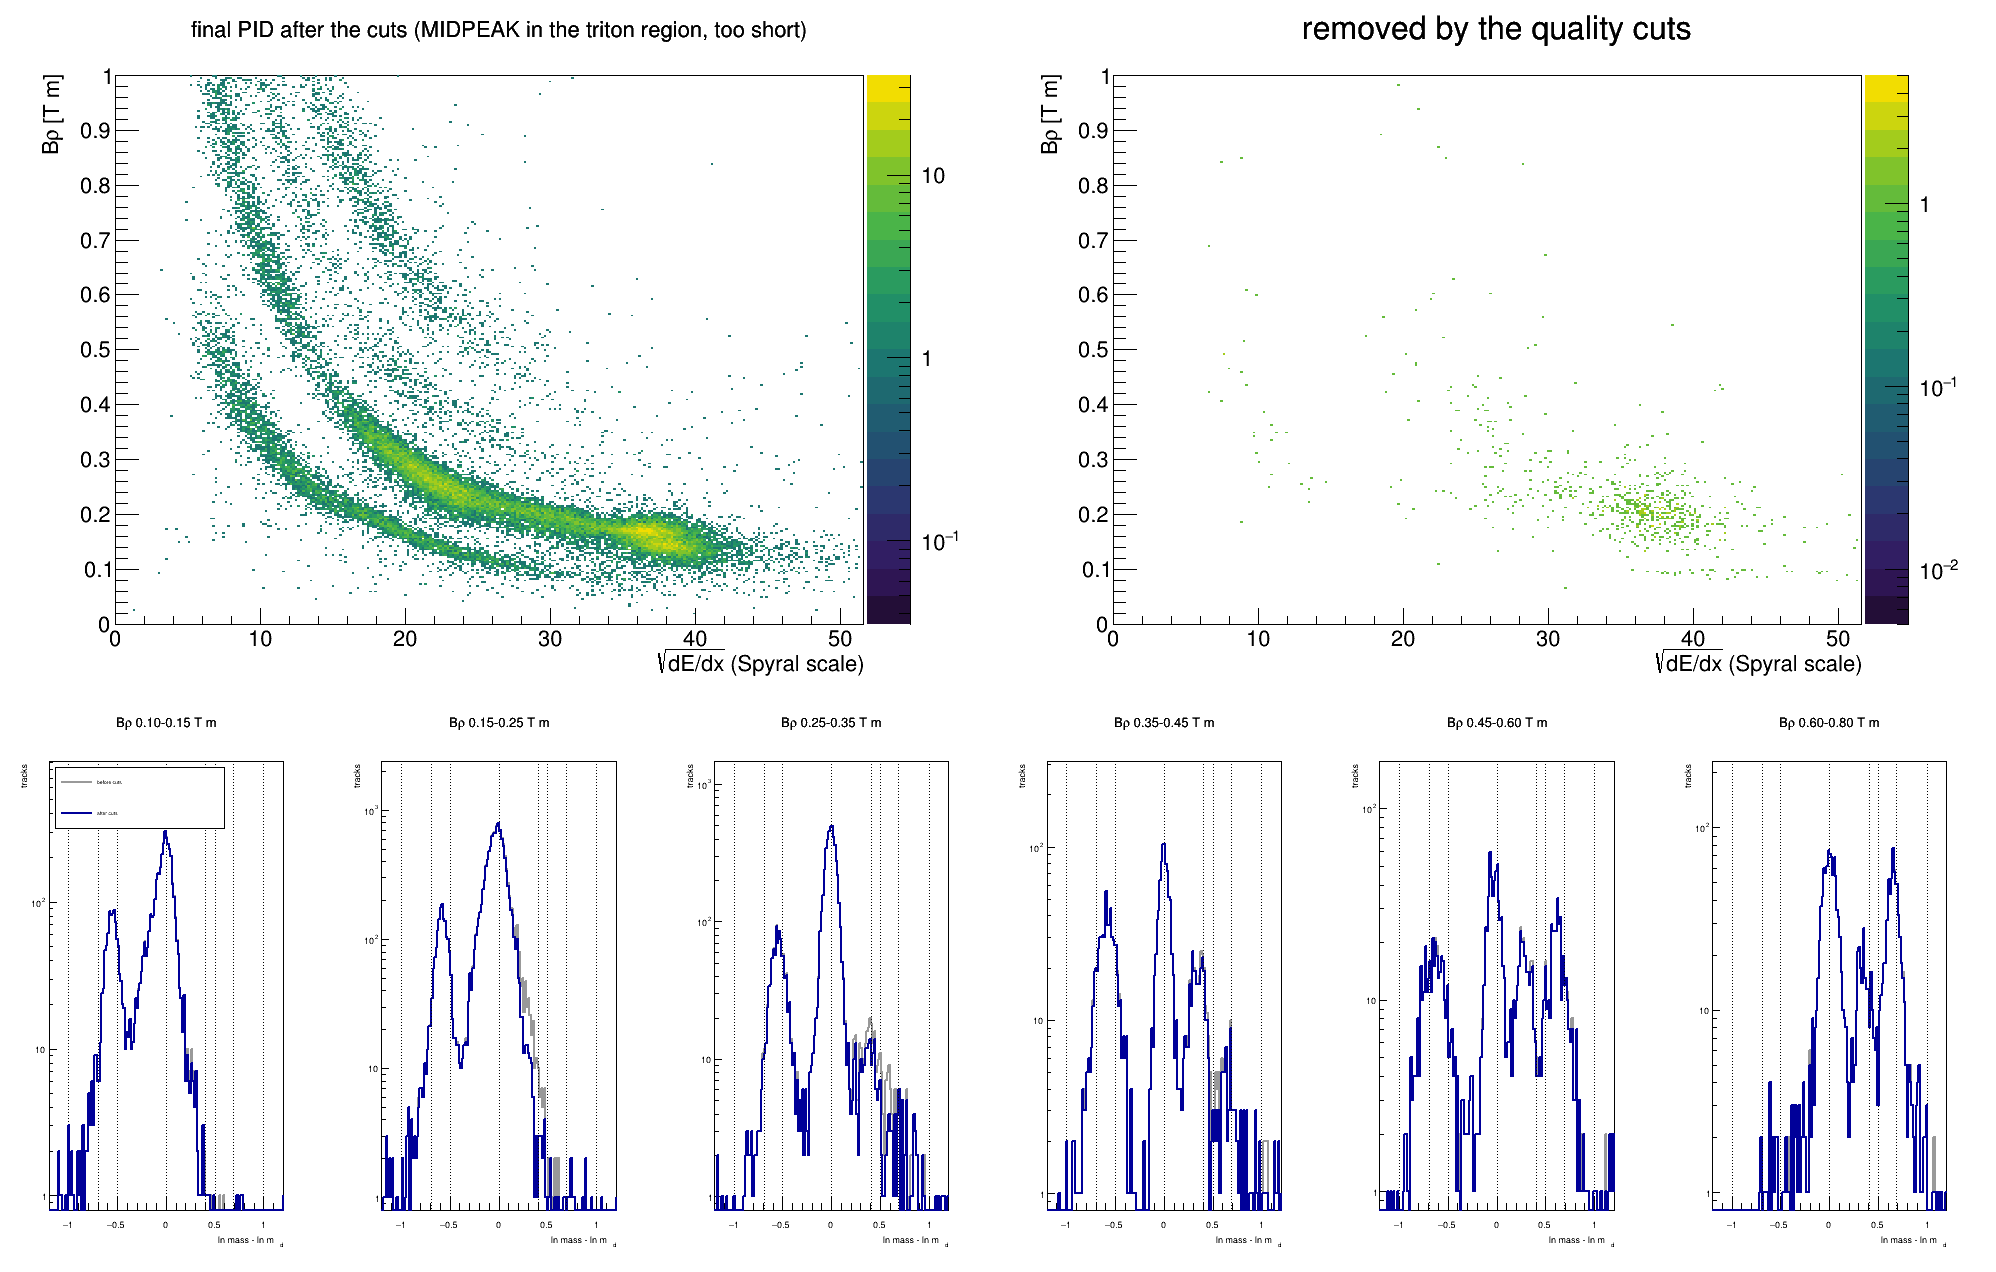
\includegraphics[width=\textwidth]{figures/pid_final_cuts_tonly.png}
  \caption{Adopted PID: the plane after the cuts and the removed tracks; bottom: ln-mass per \brho{} slice before
  (grey) and after (blue) the quality cuts.}
  \label{fig:final}
\end{figure}

\begin{table}[htbp]
  \centering
  \caption{Fraction kept by the quality cuts, data (runs 0016, 0026, 0058, 0088).}
  \label{tab:final}
  \begin{tabular}{lcc}
    \toprule
    \brho{} [T\,m] & Triton window & Deuteron peak \\
    \midrule
    0.10--0.15 & 86\,\% & 99\,\% \\
    0.15--0.25 & 40\,\% & 99\,\% \\
    0.25--0.35 & 71\,\% & 100\,\% \\
    0.35--0.45 & 91\,\% & 100\,\% \\
    0.45--0.60 & 97\,\% & 100\,\% \\
    0.60--0.80 & 100\,\% & 100\,\% \\
    \bottomrule
  \end{tabular}
\end{table}

\begin{itemize}
\item \textbf{Protons and deuterons} are cleanly separated at all \brho.
\item \textbf{Deuterons and tritons} are separated above 0.35~T\,m; $^4$He forms its own group above 0.45~T\,m and is
  as abundant as the deuterons at 0.60--0.80~T\,m. At 0.25--0.35~T\,m a triton peak exists but sits on the
  deuteron tail: in simulation about 2\,\% of the deuterons fall in the triton gate there, comparable to the triton
  population because deuterons are far more abundant. Below 0.25~T\,m there are almost no real tritons (21 of about
  7400 simulated), and most of the triton-like data tracks there are removed by the cuts.
\end{itemize}

\section{Implementation in ATTPCROOT}

All options default to off, so existing productions are unchanged. Setters:
\begin{itemize}
\item \code{AtHelix3D::SetArcAngle} -- stores \code{thetaArc} and \code{brhoArc};
\item \code{SetContainment} and \code{SetMidPeak} -- tune the flags \code{contained}, \code{rStop}, \code{zLabStop},
  \code{midPeak}, \code{peakFrac} and \code{tailRatio}, which are filled on every track;
\item \code{AtPIDTask::SetPadGainMap} -- reads the map with \code{AtPIDGainTable::LoadPadGains} and corrects a copy of
  each track;
\item \code{AtPIDTask::SetCombine} -- fills \code{AtPIDEvent::GetCombined()} (\code{AtPIDEvent} version 3) using the
  rule \code{AtTools::CombinePID}.
\end{itemize}
The a1975 configuration:
\begin{verbatim}
auto pid = new AtPIDTask();
pid->SetMinPoints(15);
pid->SetDedxGain(gSpyral, g3D);          // per run, from AtPIDGainTable
pid->SetPadGainMap("padgain_d2_v1.txt");
pid->GetHelix3D().SetHitRefit(true, true);
pid->GetHelix3D().SetArcAngle(true);
AtTools::AtPIDCombineOpt opt;            // lnRatioMax 0.25, maxBrho 0.45
opt.highSq = 30;                         // a1975 D2 units
opt.addBackScale = 0.965;                // a1975 D2
pid->SetCombine(true, opt);
\end{verbatim}
The two quality cuts depend on the species expected and stay at the analysis level, built on the stored flags.

\paragraph{Validation.} Twelve unit tests cover the arc angle, the charge-peak flag, containment, the combination
rule and the pad-map parser. On run 0026 (2670 tracks) the framework reproduces the analysis macros exactly for
\code{brhoArc}, the 3D \dedx, the veto, the charge-peak flag and containment
(\code{validate\_pid\_framework\_dp.C}). The a1975 quality cuts were derived on raw charges: with the pad map applied
the charge-peak flag changes for 4.6\,\% of the tracks and containment for 0.7\,\%. A short end-to-end run of
\code{AtPIDTask} wrote the new branch with all fields filled. The repository page
\code{docs/subsystems/pid.md} gives the same information in reference form, with a guide for choosing a PID method
in a new experiment.

\section{Open issues}
\label{sec:open}

\begin{enumerate}
\item \textbf{Saturation in the simulation.} Measure the per-pad clip level, the pedestal and the PSA response to
  clipped pulses from the data, build a per-pad ceiling map, and re-reconstruct the simulations. Until then the
  simulated \dedx{} resolution is optimistic for heavily ionizing tracks.
\item \textbf{Triton-gate purity below 0.35~T\,m.} Estimate the deuteron background under the triton peak from the
  deuteron simulation, once it includes saturation.
\item \textbf{Efficiencies.} The veto and the quality cuts must be folded into the acceptance.
\item \textbf{An unidentified population.} Short, nearly straight, heavily saturated tracks, more ionizing than
  tritons.
\item \textbf{Spyral plus veto against the circle below 0.35~T\,m.} The circle had lower deuteron leakage into the
  triton gate in simulation, but most of Spyral's leakage was the population the veto now removes; this has not been
  re-measured.
\item \textbf{Gates.} Draw the gates on the final plane, separately below and above 0.45~T\,m, where the estimators
  change.
\end{enumerate}

\appendix
\section{Macros}

All in \code{macro/Unpack\_HDF5/a1975/D2\_UKF/} unless stated.

\begin{center}
\small
\begin{tabular}{p{0.52\textwidth}p{0.42\textwidth}}
  \toprule
  Macro & Purpose \\
  \midrule
  \code{pid\_gain\_norm.C}, \code{pad\_gain\_map\_dp.C} & per-run gain, pad-gain map \\
  \code{pid\_sbpid\_dp.C} & PID trees: Spyral, 3D, arc angle, EOM, Bragg (data and simulation) \\
  \code{spiral\_fit\_dp.C} & shrinking-radius fit \\
  \code{range\_dp.C} & range, containment, charge-peak flag \\
  \code{gf\_hyp\_run\_dp.sh}, \code{gf\_hyp\_read\_dp.C}, \code{gf\_hyp\_sep\_dp.C} & genfit two-hypothesis test \\
  \code{plot\_pid\_dt\_sim\_dp.C} & deuterons and tritons from simulation in one plane \\
  \code{plot\_pid\_spyral\_veto\_dp.C}, \code{plot\_pid\_spyral\_final\_dp.C} & Spyral veto and re-add \\
  \code{plot\_pid\_range\_sim\_dp.C}, \code{plot\_pid\_range\_data\_dp.C} & range planes \\
  \code{classify\_short\_t\_dp.C}, \code{display\_short\_t\_dp.C} & short triton-like tracks \\
  \code{plot\_pid\_final\_cuts\_dp.C} & adopted PID with the quality cuts \\
  \code{validate\_pid\_framework\_dp.C} & framework against macros \\
  \code{C16\_dd\_el\_sim.C} & elastic deuteron simulation (in \code{macro/Simulation/} \code{ATTPC/16C\_dt/}) \\
  \bottomrule
\end{tabular}
\end{center}

\end{document}
